\documentclass[12pt]{article}

% Maths
\usepackage{amsmath}
\usepackage{amssymb}
\usepackage{bbm} % indicator function

% For (short)intertext
\usepackage{mathtools}

% Hyperlink
\usepackage{hyperref}
\hypersetup{
    colorlinks=true,
    linkcolor=blue,
    filecolor=magenta,      
    urlcolor=blue,
    pdfpagemode=FullScreen,
}

% Figures
\usepackage{graphics, float, subfig}
\usepackage[pdflatex]{graphicx}

% For custom environments
\usepackage{environ}

% Custom Environments
\NewEnviron{a_eq*}{\begin{center} \begin{align*} \BODY \end{align*} \end{center}}
\NewEnviron{a_eq}{\begin{center} \begin{align} \BODY \end{align} \end{center}}
\NewEnviron{c_eq*}{\begin{center} \begin{gather*} \BODY \end{gather*} \end{center}}
\NewEnviron{c_eq}{\begin{center} \begin{gather} \BODY \end{gather} \end{center}}
\NewEnviron{my_mp}{\begin{minipage}{\textwidth} \BODY \end{minipage}}

% Code
\usepackage{listings}
\usepackage{xcolor}
\definecolor{codegreen}{rgb}{0,0.6,0}
\definecolor{codegray}{rgb}{0.5,0.5,0.5}
\definecolor{codepurple}{rgb}{0.58,0,0.82}
\definecolor{backcolour}{rgb}{0.95,0.95,0.92}
\lstdefinestyle{mystyle}{
    backgroundcolor=\color{backcolour},   
    commentstyle=\color{codegreen},
    keywordstyle=\color{magenta},
    numberstyle=\tiny\color{codegray},
    stringstyle=\color{codepurple},
    basicstyle=\ttfamily\footnotesize,
    breakatwhitespace=false,         
    breaklines=true,                 
    captionpos=b,                    
    keepspaces=true,                 
    numbers=left,                    
    numbersep=5pt,                  
    showspaces=false,                
    showstringspaces=false,
    showtabs=false,                  
    tabsize=2
}
\lstset{style=mystyle}


% Itemize
\renewcommand{\labelitemi}{\textbullet}
\renewcommand{\labelitemii}{\textbullet}
\renewcommand{\labelitemiii}{\textbullet}

% Margins
\usepackage[margin=1in]{geometry}

%colors for questions
\usepackage{xcolor}

% Custom Commands
\renewcommand{\P}{\mathbb{P}}
\newcommand{\R}{\mathbb{R}}
\newcommand{\Z}{\mathbb{Z}}
\newcommand{\E}{\mathbb{E}}
\newcommand{\N}{\mathcal{N}}
\newcommand{\V}{\mathbb{V}}
\newcommand{\D}{\mathcal{D}}
\newcommand{\X}{\mathbf{X}}
\newcommand{\x}{\mathbf{x}}
\newcommand{\y}{\mathbf{y}}
\newcommand{\Y}{\mathbf{Y}}
\newcommand{\w}{\mathbf{w}}
\newcommand{\z}{\mathbf{z}}
\newcommand{\bd}{\boldsymbol{\delta}}
\newcommand{\0}{\boldsymbol{0}}
\newcommand{\1}{\boldsymbol{1}}
\renewcommand{\L}{\mathcal{L}}
\newcommand{\bq}{\bullet\quad}

% Title
\title{CSE 599B: Homework 2 Submission}
\author{Alexey Yermakov}
\date{May 6, 2024}

\begin{document}

\maketitle

\section{Policy Gradient}

\begin{itemize}
    \item The mean rewards during training with default parameters for Policy Gradient is shown below as well as Policy Gradient without normalization:

    \begin{figure}[H]
        \centering
        \begin{minipage}{0.45\textwidth}
            \centering
            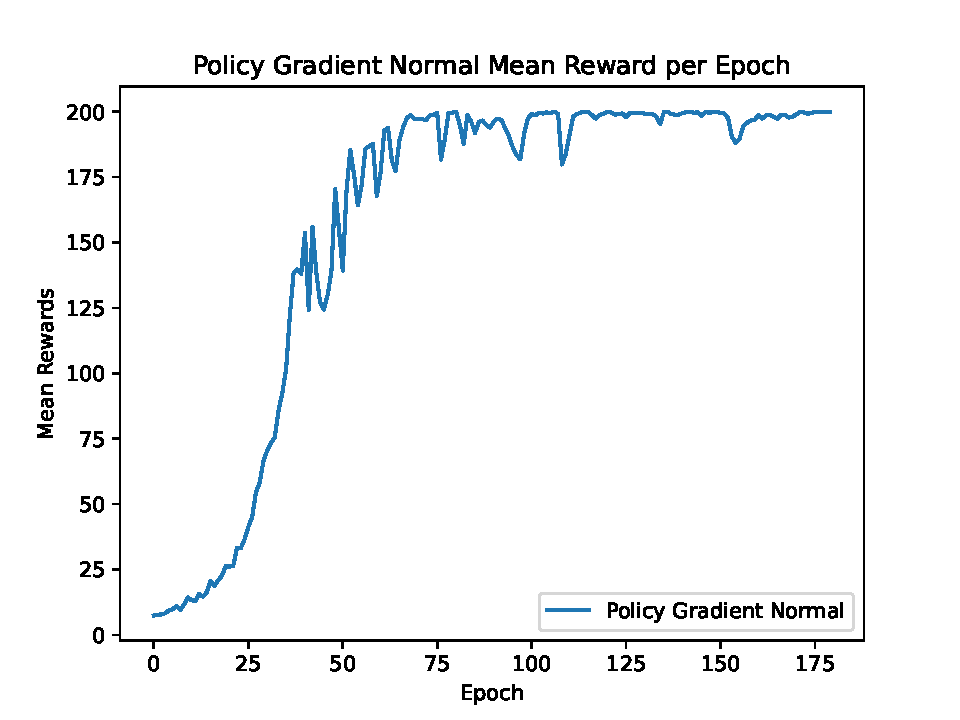
\includegraphics[width=1.0\linewidth]{../figs/pg_normal.pdf}
            \caption{Policy Gradient trained with normal hyperparameters.}
            \label{fig:fig1}
        \end{minipage}
        \hspace{0.05\linewidth}
        \begin{minipage}{0.45\textwidth}
            \centering
            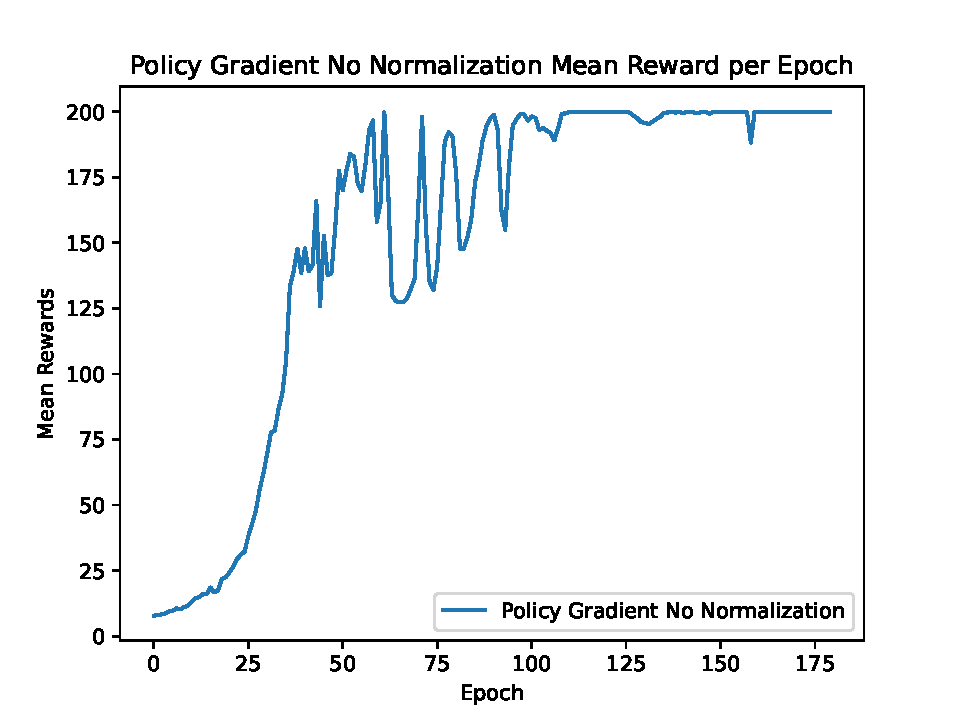
\includegraphics[width=1.0\linewidth]{../figs/pg_nonorm.pdf}
            \caption{Policy Gradient trained with no normalization.}
            \label{fig:fig2}
        \end{minipage}
    \end{figure}

    \item The success rate and average reward for Policy Gradient with normal parameters is:
    \begin{verbatim}
Success rate:  0.97
Average reward (success only):  200.0
Average reward (all):  199.58
    \end{verbatim}

    \item The success rate and average reward for Policy Gradient with no normalization is:
    \begin{verbatim}
Success rate:  1.0
Average reward (success only):  200.0
Average reward (all):  200.0
    \end{verbatim}

    \item For policy gradient for the inverted pendulum problem, it appears that the average reward is unaffected when removing the reward normalization.
    
\end{itemize}

\newpage

\section{Actor Critic}

\begin{itemize}
    \item The mean rewards during training with default parameters for Actor Critic is shown below as well as Actor Critic without a separate target Q function:

    \begin{figure}[H]
        \centering
        \begin{minipage}{0.45\textwidth}
            \centering
            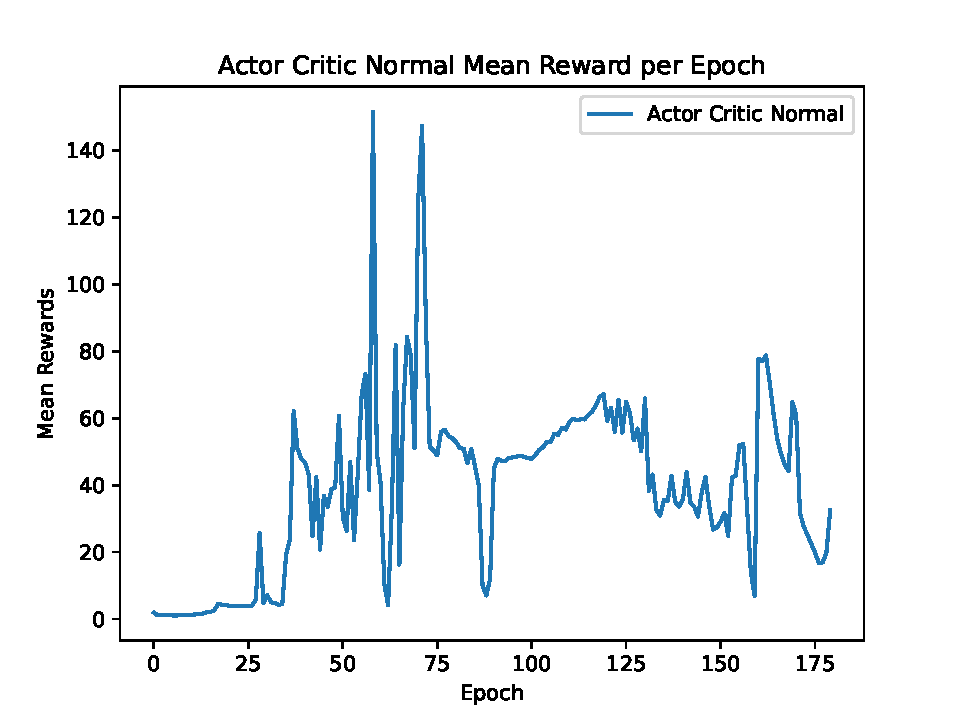
\includegraphics[width=1.0\linewidth]{../figs/ac_normal.pdf}
            \caption{Actor Critic trained with normal hyperparameters.}
            \label{fig:fig3}
        \end{minipage}
        \hspace{0.05\linewidth}
        \begin{minipage}{0.45\textwidth}
            \centering
            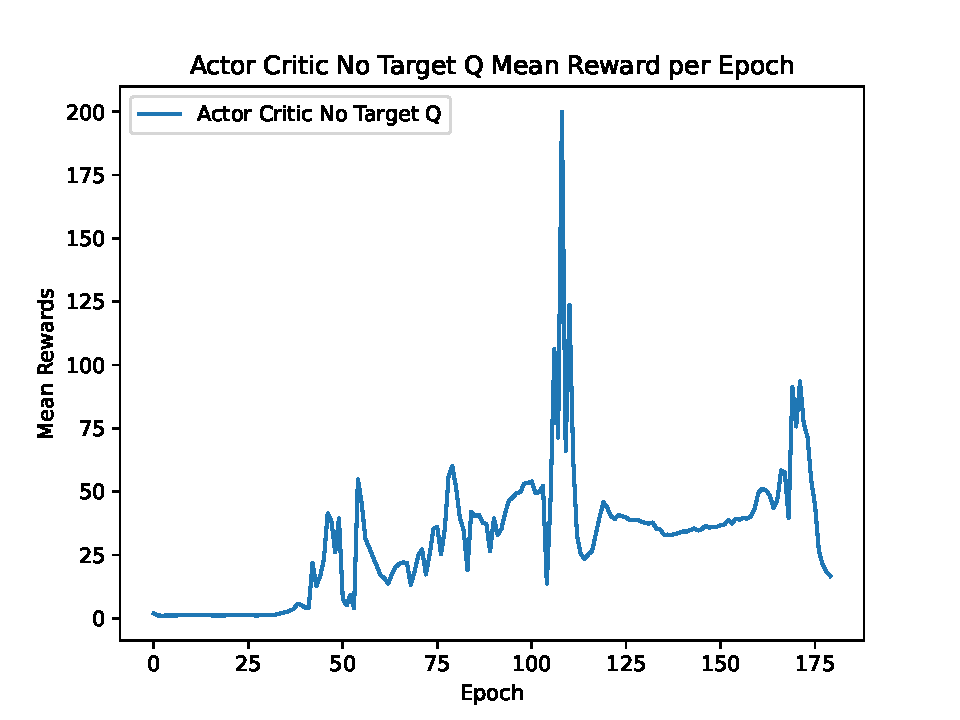
\includegraphics[width=1.0\linewidth]{../figs/ac_notarget.pdf}
            \caption{Actor Critic trained without a separate target Q function.}
            \label{fig:fig4}
        \end{minipage}
    \end{figure}

    \item The success rate and average reward for Actor Critic with normal parameters is:
    \begin{verbatim}
Success rate:  1.0
Average reward (success only):  200.0
Average reward (all):  200.0
    \end{verbatim}

    \item The success rate and average reward for Actor Critic without a separate target Q function is:
    \begin{verbatim}
Success rate:  0.0
Average reward (success only):  0.0
Average reward (all):  16.09
    \end{verbatim}

    \item For Actor Critic for the inverted pendulum problem, it appears that the average reward is completely stunted when not using a separate target Q function. This isn't shown in the average rewards plot, but is shown in the testing average reward, where the Actor Critic policy with no separate target Q function doesn't learn anything.
    
\end{itemize}

\newpage

\section{Discussion}

\begin{itemize}
    \item The role of the value function in actor-critic methods is that it enables actor-critic methods to learn off-policy and with lower variance. The off-policy learning comes from using two Q functions: one whose parameters we're updating, and the other whose parameters are fixed (and are usually set to the previous parameter values of the Q function being updated). The lower variance is a result of the gradient updates use the entire set of all previous roll-outs. Thus, actor critic methods are much more sample efficient and stable due to being able to use old information.
    \item Policy gradient, however, has to rollout new paths every time a gradient step is taken. It cannot utilize previous rollouts like actor-critic since the gradient step requires information from the current policy. Thus, policy gradient is on-policy and much less sample efficient. This also makes it significantly less stable, since it has a significantly smaller amount of data it can use due to not being able to use old information.
    \item From the above plots, its clear that the mean reward per epoch is highly variable. This is likely due to the learned Q function being only an approximation to the sum of rewards, whereas policy gradient doesn't have this approximation and instead uses monte-carlo to obtain this value.
    \item Lastly, from the above plots it appears that policy gradient seems to converge pretty well given enough epochs.
\end{itemize}

\end{document}